\chapter{\selectlanguage{greek}Ανάλυση και Σχεδίαση Συστήματος}

\section{Περιγραφή Συστήματος}

Το αντικείμενο του κεφαλαίου αυτού είναι μια λεπτομερής περιγραφή του συστήματος που αναπτύξαμε.
Σκοπός της εργασίας είναι να παρουσιάσει ένα σύστημα το οποίο 
%αναπαριστά και περιγράφει πληροφορία για τα προφίλ των χρηστών και 
επιτρέπει την εξαγωγή συμπερασμάτων για την υποστήριξη εξατομικευμένων συστάσεων για άρθρα ειδήσεων. 

Όπως έχουμε ήδη αναφέρει και σε προηγούμενο κεφάλαιο, το διαδίκτυο αυξάνεται με
γρήγορους ρυθμούς και παράλληλα αυξάνεται και η πληροφορία που περιέχεται σε αυτό, 
και συγκεκριμένα η ενημερωτική πληροφορία. Όλο και περισσότεροι χρήστες
χρησιμοποιούν το διαδίκτυο για να ενημερώνονται. Λόγω του μεγάλου όγκου των
πληροφοριών που κατακλύζουν το διαδίκτυο, οι χρήστες δυσκολεύονται να ξεχωρίσουν
τις πληροφορίες που σχετίζονται πραγματικά με τα ενδιαφέροντά τους. 
Η παραπάνω κατάσταση δημιουργεί ένα σημαντικό πρόβλημα για τους χρήστες του διαδικτύου σε
καθημερινή βάση.\\
Η διαρκής ροή ειδήσεων από διάφορες πηγές ενημέρωσης δεν εξυπηρετεί τον χρήστη,
καθώς καθιστά αδύνατη την παρακολούθησή τους και κρίνεται επιβεβλημένη η
προσωποποίηση του αποτελέσματος. Σε ένα τέτοιο σενάριο τα συστήματα συστάσεων
μπορούν να αντιμετωπίσουν το πρόβλημα, προτείνοντας αντικείμενα που
προηγουμένως ήταν άγνωστα, στην περίπτωσή μας άρθρα ειδήσεων, και θα
ενδιέφεραν έναν συγκεκριμένο χρήστη. Τυπικά, τέτοια συστήματα χρησιμοποιούν
προφίλ χρηστών και έχουν σαν στόχο τη σύσταση ειδήσεων που ταιριάζουν καλύτερα
στο προφίλ αυτό.\\

Στο σύστημά μας τα άρθρα ειδήσεων λαμβάνονται από το διαδίκτυο από αρκετές υπηρεσίες ειδήσεων, 
καθώς και από τη συλλογή άρθρων {\textit {{\en {Reuters}}} του {\en {NLTK (Natural Language Toolkit)}}. 
Τα άρθρα αποθηκεύονται στη βάση δεδομένων του συστήματος και 
το σύστημα επεξεργάζεται το περιεχόμενο κάθε άρθρου που είναι αποθηκευμένο στη βάση. 

% ++++++++++++++++++++++++++++++

Στη συνέχεια, το λειτουργικό μέρος το οποίο πραγματοποιεί την δημιουργία του προφίλ δέχεται σαν είσοδο τις
προτιμήσεις του χρήστη. 
Ο μηχανισμός προτάσεων του συστήματος παράγει ένα σύνολο εξατομικευμένων προτάσεων που
παρουσιάζει στον χρήστη.
\\

Παρακάτω, παρουσιάζεται η μελέτη που έγινε για την υλοποίηση του συστήματος συστάσεων. 
Αρχικά, παρουσιάζεται η αρχιτεκτονική του συστήματος και γίνεται ο διαχωρισμός του στα επιμέρους υποσυστήματα 
και εν συνεχεία, αναλύεται λεπτομερώς ο τρόπος λειτουργίας των υποσυστημάτων του.

\section{Αρχιτεκτονική Συστήματος}
% Ανάλυση - Περιγραφή 

Στην ενότητα αυτή παρουσιάζεται ο χωρισμός του συστήματος συστάσεων σε υποσυστήματα όσον αφορά την αρχιτεκτονική.
\newpage
Η αρχιτεκτονική που χρησιμοποιήθηκε για το σύστημά μας παρουσιάζεται στο παρακάτω σχήμα:

\begin{figure}[!ht] \centering
    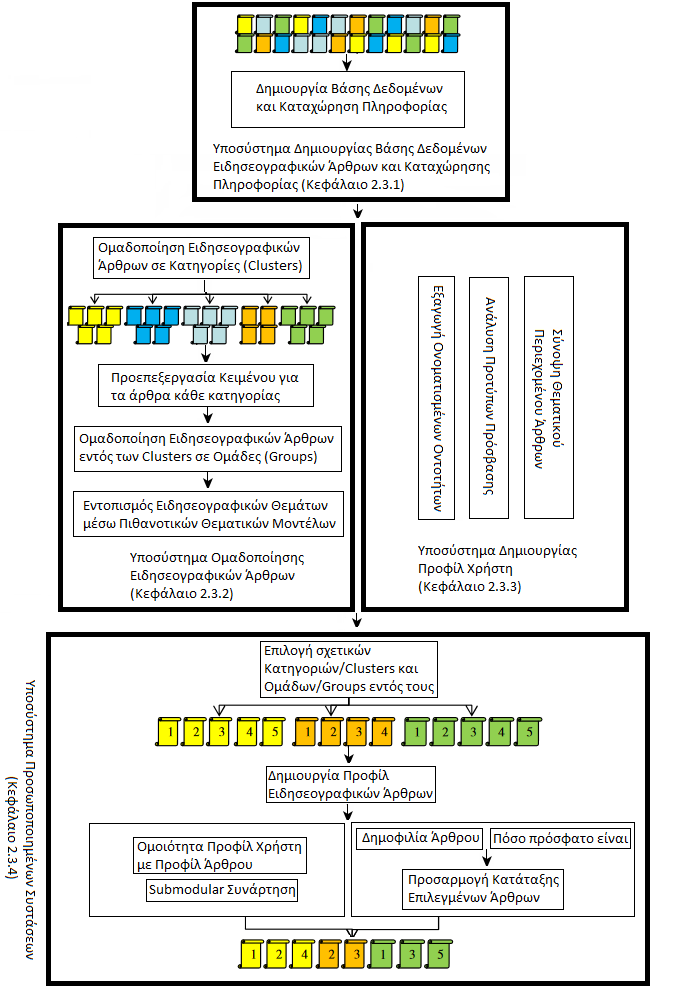
\includegraphics[scale=0.77]{static/figures/arch1.png}
    \caption{Αρχιτεκτονική Συστήματος}
    \label{}
\end{figure} 

\section{Υποσυστήματα}

Στη συνέχεια παρουσιάζουμε τα διάφορα υποσυστήματα από τα οποία αποτελείται ο
μηχανισμός προκειμένου να γίνει κατανοητή η λειτουργία του.

\begin{enumerate}

  \item Υποσύστημα Δημιουργίας Βάσης Δεδομένων και Καταχώρησης Πληροφορίας
    \begin{itemize}
      \item{Συλλογή Ειδησεογραφικών Άρθρων}
      \item{Δημιουργία Βάσης Δεδομένων και Καταχώρηση Πληροφορίας}
      \end{itemize}
  
  \item Υποσύστημα Ομαδοποίησης Ειδησεογραφικών Άρθρων
    \begin{itemize}
    \item{Ομαδοποίηση Ειδησεογραφικών Άρθρων σε Κατηγορίες {\en {(Clusters)}}}
    \item{Προεπεξεργασία Κειμένου {\en {(Text Preprocessing)}}}
    \item{Ομαδοποίηση Ειδησεογραφικών Άρθρων εντός των {\en {Clusters}} σε Ομάδες {\en {(Groups)}}}
    \item{Εντοπισμός Ειδησεογραφικών Θεμάτων μέσω Πιθανοτικών Θεματικών Μοντέλων}
  \end{itemize}
  
  \item Υποσύστημα Δημιουργίας Προφίλ Χρήστη
    \begin{itemize}
      \item Σύνοψη Θεματικού Περιεχομένου Άρθρων
      \item Ανάλυση Προτύπων Πρόσβασης
      \item Εξαγωγή Ονοματισμένων Οντοτήτων
    \end{itemize}

  \item Υποσύστημα Προσωποποιημένων Συστάσεων
    \begin{itemize}
     \item Αντιστοίχιση Αναγνωστικών Προτιμήσεων για την Αναπαράσταση 1ου Επιπέδου
     \item Αντιστοίχιση Αναγνωστικών Προτιμήσεων για την Αναπαράσταση 2ου Επιπέδου
     \begin{enumerate}
      \item Δημιουργία Προφίλ Ειδησεογραφικών Άρθρων
      \item Εισαγωγή στις {\en {Submodular}} Συναρτήσεις
      \item Μοντέλο Συστάσεων
      \item Προσαρμογή Κατάταξης Ειδησεογραφικών Άρθρων
      \end{enumerate}
    \end{itemize}

\end{enumerate}

Παρακάτω δίνεται λεπτομερής περιγραφή για καθένα από τα υποσυστήματα που αναφέραμε.

% **********************************************************
\subsection{Υποσύστημα Δημιουργίας Βάσης Δεδομένων και Καταχώρησης Πληροφορίας}
% **********************************************************

Η συλλογή των άρθρων ανακτήθηκε κατά βάση από το διαδίκτυο από αρκετές διαδικτυακές υπηρεσίες ειδήσεων, 
όπως οι εξής: {\textit {{\en {The Guardian, New York Times, Washington Post, Fox News, Independent, Reuters, Sky News}}}. 
Ένα μέρος της συλλογής προήλθε από τη συλλογή άρθρων {\textit {{\en {Reuters}}} του {\en {NLTK}}.

Μετά την ολοκλήρωση της διαδικασίας συλλογής, 
δημιουργούμε τη βάση δεδομένων και αποθηκεύουμε τα άρθρα στους αντίστοιχους πίνακες της βάσης του συστήματος.
Οι πληροφορίες που αποθηκεύονται για κάθε άρθρο είναι: 
τίτλος, συγγραφέας, ημερομηνία δημοσίευσης, κείμενο άρθρου, γενική κατηγορία ({\en {cluster}}) στην οποία ανήκει το κάθε άρθρο. \\
Επιπρόσθετα, στο αρχικό αυτό στάδιο, δημιουργούμε και καταχωρούμε μία σειρά από χρήστες του συστήματος. 
Συγκεκριμένα, κατά τη δημιουργία της βάσης δεδομένων παράγεται αυτόματα ένα αναγνωστικό ιστορικό για κάθε αποθηκευμένο χρήστη, 
τόσο ελεγχόμενα όσο και τυχαία και αποθηκεύεται στον αντίστοιχο πίνακα της βάσης. 
Ως προς το ελεγχόμενο μέρος επιχειρούμε να ταιριάξουμε κάθε αποθηκευμένο χρήστη με μία συγκεκριμένη κατηγορία άρθρων, 
φορτώνοντας στο αναγνωστικό ιστορικό του μέσω ενός αρχείου μεγαλύτερο αριθμό άρθρων από κάποια συγκεκριμένη κατηγορία. 
Μέσω του ελεγχόμενου τρόπου καταφέρνουμε να διασφαλίσουμε ότι κάθε άρθρο της βάσης δεδομένων θα έχει αναγνωσθεί 
τουλάχιστον μία φορά από κάποιον τυχαίο χρήστη.
Ως προς το τυχαίο μέρος επιλέγουμε μέσω της συνάρτησης {\en {\textit{rand}} και έναν τυχαίο (εντός ορίων) αριθμό άρθρων από οποιαδήποτε κατηγορία 
για να εμπλουτίσουμε το περιεχόμενο του αναγνωστικού ιστορικού του χρήστη. \\

Πλέον, έχουμε συλλέξει στη βάση δεδομένων όλη την απαραίτητη πληροφορία για το επόμενο υποσύστημα.

% **********************************************************
\subsection{Υποσύστημα Ομαδοποίησης Ειδησεογραφικών Άρθρων}
% **********************************************************

Τυπικά, δεδομένου ενός σετ ειδησεογραφικών άρθρων {\en {\textit{N = \{$n_1, n_2, ..., n_M$\}}}}, 
όπου {\en {\textit{$\vert N\vert$ = M}}}, στόχος μας είναι μια στιβαρή ομαδοποίηση {\en {(hard clustering)
C = \{$C_1, C_2, ..., C_K$\}}} στο {\en {\textit{N}}, όπου το {\en {\textit{K}} είναι ένας προκαθορισμένος 
αριθμός από {\en {clusters}}. Κάθε {\en {cluster}} {\en {\textit{$C_i$}}} αποτελείται από μία λίστα από {\en {groups}} 
ειδησεογραφικών άρθρων {\en {G = \{$G_1, G_2, ...$\}}} και κάθε {\en {group}} {\en {\textit{$G_j$}}} 
περιέχει {\en {\textit{$t_j$}}} ειδησεογραφικά άρθρα. 
Κάθε {\en {cluster}} καθώς και τα {\en {groups}} άρθρων που περιλαμβάνει είναι αντιστοίχως συσχετισμένα 
με μία κατανομή θεμάτων {\en {\textit{T}}}, η οποία περιγράφει τα θέματα που “κρύβονται” μέσα στα άρθρα. 
Στόχος της συγκεκριμένης αναπαράστασης είναι ο εξής: 
Οι προσωποποιημένες συστάσεις άρθρων απαιτούν γρήγορη απόκριση για να παρουσιάσουν 
άμεσα αποτελέσματα στους χρήστες. Η συγκεκριμένη αναπαράσταση άρθρων μπορεί να βοηθήσει 
στη γρήγορη πλοήγηση προς άρθρα που ενδιαφέρουν το χρήστη. 

% ____________________________________________
\subsubsection{Ομαδοποίηση Ειδησεογραφικών Άρθρων σε Κατηγορίες {\en {(Clusters)}}}
% ____________________________________________

Δεδομένου του τρόπου συλλογής των άρθρων που βρίσκονται αποθηκευμένα στη βάση δεδομένων του συστήματος, 
γνωρίζουμε εκ των προτέρων την κατηγορία στην οποία ανήκουν το κάθε ένα από αυτά. 
Έτσι, είτε πρόκειται για άρθρα που προέρχονται από διαδικτυακές υπηρεσίες ειδήσεων, 
είτε για άρθρα από τη συλλογή {\en {Reuters}} του {\en {NLTK}}, κάθε ένα είναι εξαρχής συσχετισμένο 
με μια συγκεκριμένη κατηγορία από το σύνολο των διαφορετικών κατηγοριών που έχουμε επιλέξει. \\
Στο σύστημά μας εμφανίζονται άρθρα από εφτά διαφορετικές κατηγορίες. 
Κάθε κατηγορία σχετίζεται με ένα από τα παρακάτω θέματα: 
\textit{{\en {Science/Technology, Politics, Sports, Life \& Style, Sugar, Coffee, Housing}}}. 
Οι τέσσερις πρώτες κατηγορίες περιλαμβάνουν άρθρα που συλλέχθηκαν από το διαδίκτυο, 
ενώ οι υπόλοιπες τρεις κατηγορίες αποτελούνται από άρθρα της συλλογής {\en {Reuters}}.\\
Σε αυτό το στάδιο της προεπεξεργασίας της συλλογής κειμένων μπορούμε να θεωρήσουμε με βεβαιότητα 
ότι αυτή η πρώτη ομαδοποίηση που πραγματοποιήθηκε πάνω στη συλλογή κειμένων είναι και η πιο αποτελεσματική, 
καθώς έχουμε εξασφαλίσει ότι τα ειδησεογραφικά άρθρα με κοινό θεματικό περιεχόμενο ανήκουν στο ίδιο {\en {cluster}}. \\
Τέλος, είναι σαφές ότι κάθε άρθρο ανήκει αποκλειστικά σε ένα και μοναδικό {\en {cluster}}. 
\\

Παρακάτω προχωρούμε σε περαιτέρω ομαδοποίηση των άρθρων, αυτή τη φορά εντός των {\en {clusters}} που δημιουργήσαμε, 
με σκοπό τη δημιουργία της βάσης του πρώτου επιπέδου σύστασης ειδησεογραφικών άρθρων του συστήματός μας. 

% ____________________________________________
\subsubsection{Προεπεξεργασία Κειμένου {\en {(Text Preprocessing)}}}
% ____________________________________________

Πρωτού προβούμε σε εφαρμογή του αλγορίθμου ομαδοποίησης των άρθρων εντός των  {\en {clusters}} σε ομάδες {\en {(groups)}}, 
κρίνεται απαραίτητη η προεπεξεργασία των κειμένων των άρθρων κάνοντας χρήση της βιβλιοθήκης {\en {scikit-learn}} της {\en {Python}}. 
Η πληροφορία που δίνεται σαν είσοδος στο μηχανισμό προέρχεται από τη βάση δεδομένων του συστήματος 
και αποτελείται από τα κείμενα των άρθρων κάθε {\en {cluster}}. 
Πρωταρχικός σκοπός μας στο στάδιο αυτό είναι η απομάκρυνση ανεπιθύμητων συμβολοσειρών μέσω φιλτραρίσματος των λέξεων 
που δε φέρουν ουσιαστική πληροφορία και η ανάλυση του κειμένου για την εξαγωγή λέξεων-κλειδιών από το κείμενο του κάθε άρθρου.
Βασικά σημεία προεπεξεργασίας: 
\begin{itemize}
 \item \textbf{Λεξική Ανάλυση}: Το στάδιο αυτό αφορά τον διαμερισμό κάθε άρθρου στα συστατικά στοιχεία του κειμένου του {\en {(tokenization)}}, 
 μετατρέποντας το κείμενο σε ακολουθία λέξεων. 
 \item \textbf{Αφαίρεση τετριμμένων λέξεων και τερματικών όρων {\en {(stopwords)}}}: Για κάθε άρθρο της συλλογής πραγματοποιείται καθαρισμός 
 από τετριμμένες λέξεις {\en {(elimination of insignificant words)}}, 
όπως είναι τα άρθρα, οι σύνδεσμοι, οι αντωνυμίες, καθώς και οι συχνά χρησιμοποιούμενες λέξεις 
που δεν ανήκουν στις ανωτέρω κατηγορίες, αλλά δεν φέρουν καμία ιδιαίτερη σημασιολογική πληροφορία, 
όπως είναι ορισμένα επιρρήματα. Ένα {\en {stopword}} είναι μια συχνά χρησιμοποιούμενη λέξη, 
όπως οι {\en {``the'', ``and'', ``to'', ``also''}}, όπου μία μηχανή αναζήτησης έχει σχεδιαστεί να αγνοεί, 
τόσο κατά την ευρετηρίαση των καταχωρήσεων προς αναζήτηση, όσο και κατά την ανάκτησή τους ως αποτελέσματα μιας αναζήτησης. 
Δεν επιθυμούμε αυτές οι λέξεις να καταλαμβάνουν χώρο στη βάση δεδομένων 
ή να κατασπαταλούν πολύτιμο υπολογιστικό χρόνο, καθότι φέρουν ελάχιστον λεκτικό 
περιεχόμενο και η παρουσία τους σε ένα κείμενο δε διευκολύνει τη διάκριση του κειμένου από άλλα κείμενα. 
Το {\en {NLTK}} περιέχει μία λίστα από {\en {stopwords}} αποθηκευμένα σε δεκαέξι διαφορετικές γλώσσες.
Στο σημείο αυτό απομακρύνουμε, επίσης, τα αριθμητικά δεδομένα και τα σημεία στίξης.
 \item \textbf{Κανονικοποίηση των λέξεων}: Το στάδιο αυτό αφορά την αναγνώριση των ριζών των λέξεων, 
 γνωστή ως λημματοποίηση {\en {(lemmatization)}} και την αποκατάληξη {\en {(stemming)}}, 
ώστε να μην επηρεάζεται η εξαγωγή χαρακτηριστικών γνωρισμάτων των κειμένων από την πτώση ή το χρόνο που κλίνονται οι λέξεις. 
Έτσι, καταλήγουμε σε αναγωγή όλων των μορφολογικών τύπων μίας λέξης σε μία ενιαία αναπαράσταση. 
\item \textbf{Επιλογή των αντιπροσωπευτικών όρων}: Στη συνέχεια, η διαδικασία βασίζεται στην εξαγωγή χαρακτηριστικών γνωρισμάτων (λέξεων–κλειδιών) των κειμένων, η οποία αφορά την
εφαρμογή μέτρων ποιότητας για την επιλογή διατήρησης ορισμένων όρων για κάθε κείμενο. 
Η εξαγωγή των λέξεων–κλειδιών των κειμένων γίνεται μέσω του εργαλείου {\en {TfidfVectorizer}} \cite{Tfidf01}
της βιβλιοθήκης {\en {scikit-learn}} της {\en {Python}}. Η εξαγωγή των σωστών λέξεων-κλειδιών είναι πολύ σημαντική. \\
Η μέθοδος \textbf{{\en {TF–IDF}}} \cite{Tfidf02} είναι μια μετρική που δηλώνει πόσο σημαντικός είναι ένας όρος σε ένα έγγραφο από μια συλλογή εγγράφων. 
Η μέθοδος {\en {TF–IDF}} στοχεύει στο να σταθμίσει όλους τους όρους μιας συλλογής κειμένων. 
Με λίγα λόγια, στόχος της είναι να αποδώσει το αντίστοιχο βάρος σε κάθε όρο και, κατά επέκταση, σε κάθε διάσταση του πολυδιάστατου αυτού χώρου. 
Αυτό συμβαίνει γιατί η απλή αρίθμηση ενός όρου σε ένα κείμενο δεν αρκεί για να μας πληροφορήσει 
για τη σημαντικότητα του όρου αυτού και τη βαρύτητα της πληροφορίας που περιέχει. \\
Η μέθοδος αυτή αποτελείται από τις ποσότητες {\en {TF}} και {\en {IDF}}. 
Η ποσότητα {\en {TF}} (συχνότητα όρου) υποδηλώνει το πόσες φορές εμφανίζεται ένας όρος σε ένα κείμενο. 
Από την άλλη, η ποσότητα {\en {IDF}} υποδηλώνει το πόσο ένας όρος είναι διαδεδομένος σε 
ένα κείμενο αλλά και σε ολόκληρη τη συλλογή κειμένων. 
Τελικά, το βάρος ενός όρου προκύπτει από τον πολλαπλασιασμό των ποσοτήτων {\en {TF}} και {\en {IDF}}. \\
Στόχος της μεθόδου αυτής μέσω του βάρους είναι η επιλογή εκείνων των όρων που αποτυπώνουν καλύτερα το περιεχόμενο ενός κειμένου.
Για τον προσδιορισμό του βάρους ενός όρου είναι εξίσου σημαντικές και οι δύο ποσότητες 
{\en {TF}} και {\en {IDF}}.
Αυτό επισημαίνεται διότι αν χρησιμοποιούσαμε μόνο τη συχνότητα εμφάνισης ενός όρου ({\en {TF}}) ως βάρος,
αυτό θα είχε ως συνέπεια οι συχνότερα εμφανιζόμενοι όροι να θεωρούνται ως οι πιο σημαντικοί. 
Αυτή η υπόθεση θα μπορούσε να μας οδηγήσει σε λανθασμένη επιλογή 
όρων οι οποίοι εμφανίζονται σε πολλά κείμενα και δεν προσφέρουν κάποια ιδιαίτερη πληροφορία σε ένα κείμενο. 
Για παράδειγμα, η λέξη «εξόρυξη» σε μία συλλογή κειμένων με θέμα «Τεχνικές Εξόρυξης Κειμένων» 
θα εμφανίζεται με μεγάλη συχνότητα σε όλα τα κείμενα της συλλογής. 
Επομένως, μέσα από αυτό το παράδειγμα καταλαβαίνουμε πως ένας τέτοιος όρος, παρότι θα μπορούσε 
να εμφανίζεται αρκετές φορές σε ένα κείμενο, δε θα μπορούσε να θεωρηθεί ως ένας σημαντικός όρος,
γιατί δεν προσφέρει ένα ιδιαίτερο χαρακτηριστικό στο  κείμενο σε σχέση με τα υπόλοιπα κείμενα της συλλογής.
Εδώ, λοιπόν, καταλαβαίνουμε τη σημαντικότητα της ποσότητας {\en {IDF}} στον υπολογισμό του βάρους ενός όρου. 
Όταν ένας όρος εμφανίζεται σε πολλά κείμενα της συλλογής, η τιμή της ποσότητας {\en {IDF}} είναι μικρή, 
ενώ όταν ένας όρος εμφανίζεται σε λίγα κείμενα της συλλογής, η τιμή της ποσότητας {\en {IDF}} είναι μεγάλη. \\
Επομένως, μεγάλο βάρος για έναν όρο προκύπτει όταν ο όρος αυτός εμφανίζεται πολλές φορές σε ένα κείμενο 
και λιγότερες φορές στο σύνολο των κειμένων. \\
\end{itemize}

Χρησιμοποιώντας τη διαδικασία που περιγράψαμε παραπάνω, ο μηχανισμός διαβάζει
καινούργια άρθρα από τη βάση δεδομένων του συστήματος ανά κατηγορία {\en {(cluster)}}, 
εξάγει τις λέξεις–κλειδιά για κάθε άρθρο της κατηγορίας και τις συσχετίζει με το άρθρο και το αντίστοιχο βάρος. 
Έχοντας ολοκληρώσει την προεπεξεργασία των κειμένων της συλλογής, 
τα δεδομένα μας έχουν πλέον την κατάλληλη μορφή ώστε να προχωρήσουμε στη διαδικασία ομαδοποίησης 
των άρθρων εντός της κάθε κατηγορίας {\en {(cluster)}}. 

% ____________________________________________
\subsubsection{Ομαδοποίηση Ειδησεογραφικών Άρθρων εντός των {\en {Clusters}} σε Ομάδες {\en {(Groups)}}}
% ____________________________________________

\par Τα ειδησεογραφικά άρθρα που περιέχονται σε κάθε {\en {cluster}} επικεντρώνονται σε παρόμοιες πτυχές ενός γενικού θέματος, 
εκείνου που αντιπροσωπεύεται από τον τίτλο της εκάστοτε κατηγορίας. 
Τυπικά, ένας χρήστης ενδιαφέρεται για συγκεκριμένες πτυχές ενός θέματος και όχι για όλες. 
Βασισμένοι σε αυτή την παραδοχή και με στόχο την γρήγορη πλοήγηση, κατά το στάδιο σύστασης, προς άρθρα που ενδιαφέρουν το χρήστη, 
προχωρούμε σε περαιτέρω ομαδοποίηση των άρθρων εντός κάθε κατηγορίας με σκοπό τη δημιουργία ομάδων {\en {(groups)}} εντός κάθε {\en {cluster}}. \\

% sklearn.cluster KMeans
H ομαδοποίηση εντός κάθε {\en {cluster}} πραγματοποιείται με εφαρμογή του αλγορίθμου {\en {k-means}} με βάση κάποιο μέτρο ομοιότητας, 
με στόχο όλα τα άρθρα που ανήκουν στην ίδια ομάδα να είναι παρόμοια μεταξύ τους. 
Για την εφαρμογή του αλγορίθμου γίνεται χρήση της βιβλιοθήκης {\en {scikit-learn}} της {\en {Python}}. \\

\par O αλγόριθμος \textbf{{\en {k-means}}} \cite{Km01} είναι ο πιο διαδεδομένος αλγόριθμος ομαδοποίησης. 
O {\en {k-means}} διασπάει τα δεδομένα σε {\en {k}} διαφορετικές ομάδες μέσω μίας επαναληπτικής διαδικασίας, 
όπου {\en {k}} είναι ένας προκαθορισμένος ακέραιος αριθμός και παρέχεται από εμάς. 
Η επαναληπτική διαδικασία τερματίζει τη στιγμή που θα ικανοποιηθεί ένα συγκεκριμένο κριτήριο. 
Τα κύρια βήματα του αλγορίθμου περιγράφονται παρακάτω: 

\begin{enumerate}
 \item Αρχικά, γίνεται η επιλογή {\en {k}} σημείων στο πεδίο των δεδομένων έτσι ώστε τα σημεία αυτά 
 να αποτελούν τα κέντρα των αρχικών ομάδων. 
 \item Ανάθεσε κάθε δεδομένο σε μία ομάδα για το οποίο η απόστασή του από το κέντρο της ομάδας να είναι 
 η μικρότερη από κάθε άλλη εκ των κέντρων των υπολοίπων ομάδων. 
 \item Όταν όλα τα δεδομένα έχουν ανατεθεί στις ομάδες, υπολόγισε ξανά τα κέντρα των ομάδων, παίρνοντας 
 το μέσο όρο των δεδομένων κάθε ομάδας. 
 \item Επανάλαβε τα βήματα 2, 3 μέχρι να επαληθευτεί κάποιο κριτήριο σύγκλισης.
\end{enumerate}

Το κριτήριο σύγκλισης του αλγορίθμου, ο τρόπος μέτρησης της απόστασης των δεδομένων από τα κέντρα των ομάδων, 
καθώς και ο τρόπος ανάδειξης των αρχικών κέντρων τους καθορίζουν σε μεγάλο βαθμό την τελική ομαδοποίηση των δεδομένων 
και ορίζονται από το χρήστη. \\

% Μετά από δοκιμές με σκοπό την ανεύρεση του καταλληλότερου αριθμού k

% ********************************* +++

Τα ήδη υπάρχοντα {\en {clusters}} μαζί με τα παραγόμενα {\en {groups}} που περιέχονται σε αυτά 
αποτελούν τη βάση του πρώτου επιπέδου σύστασης ειδησεογραφικών άρθρων του συστήματός μας. 

% ____________________________________________
\subsubsection{Εντοπισμός Ειδησεογραφικών Θεμάτων μέσω Πιθανοτικών Θεματικών Μοντέλων}
% ____________________________________________

Ένας φυσικός τρόπος να εξερευνήσουμε τους συσχετισμούς μεταξύ των {\en {clusters} (ή των {\en {groups}) άρθρων 
και του προφίλ του δοθέντος χρήστη είναι να συγκρίνουμε την ομοιότητα των θεμάτων που “κρύβονται” μέσα στα άρθρα τους. 
Γενικά, η ανακάλυψη κρυμμένων θεμάτων που υπάρχουν σε μια συλλογή κειμένων πραγματοποιείται χρησιμοποιώντας 
πιθανοτικά μοντέλα θεμάτων, όπως τα {\en {PLSI}} και {\en {LDA}} \cite{Lda02}, εξάγοντας μια λίστα αντιπροσωπευτικών λέξεων 
από την αρχική συλλογή κειμένων μαζί με το αντίστοιχο βάρος για κάθε λέξη. 
Τα μοντέλα θεμάτων μοντελοποιούν κάθε αντικείμενο μιας συλλογής ως ένα πεπερασμένο μείγμα από ένα σύνολο θεματικών πιθανοτήτων. \\

Ένα γενετικό {\en {(generative)}} μοντέλο θεμάτων βασίζεται στους απλούς πιθανοτικούς κανόνες επιλογής {\en {(sampling)}} 
που περιγράφουν πως οι λέξεις μέσα στα κείμενα μπορεί να δημιουργηθούν μέσω τυχαίων κρυφών μεταβλητών. 
Όταν προσαρμόζουμε ένα γενετικό μοντέλο, ο στόχος είναι να βρεθεί το καταλληλότερο σύνολο κρυφών μεταβλητών 
που μπορεί να εξηγήσει τα παρατηρούμενα δεδομένα υποθέτοντας ότι το μοντέλο δημιουργήθηκε από τα δεδομένα. 
Το Σχήμα \ref{fig:ldamodel01} δείχνει την προσέγγιση μοντέλων θεμάτων με δύο τρόπους: 
σαν γενετικό μοντέλο και σαν πρόβλημα μεταβολικής συμπερασματολογίας. 
Στα αριστερά, η γενετική διαδικασία παρουσιάζεται με δύο θέματα {\en {(topics)}}. 
Τα {\en {Topic}} 1 και 2 είναι θεματικά συσχετισμένα με το {\en {'money'}} και τα {\en {'rivers'}} 
και απεικονίζονται σαν τσάντες που περιέχουν διαφορετικές κατανομές ως προς τις λέξεις. 
Διαφορετικά κείμενα μπορούν να παραχθούν επιλέγοντας λέξεις από ένα θέμα δεδομένου του βάρους που έχει. 
Για παράδειγμα, τα κείμενα {\en {Doc1}} και {\en {Doc3}} έχουν δημιουργηθεί με την διαδικασία \textit{{\en {sampling}}} 
μόνο από το {\en {topic}} 1 και το {\en {topic}} 2 αντίστοιχα, 
ενώ το κείμενο {\en {Doc2}} δημιουργήθηκε από την ίση μείξη των δύο θεμάτων. 
Με τον τρόπο όπου το μοντέλο ορίστηκε, δεν υπάρχει κάποια αμοιβαία αποκλειστικότητα 
που να περιορίζει τις λέξεις να είναι μέρος ενός μόνο θέματος. 
Αυτό επιτρέπει στο μοντέλο να καταλαβαίνει την πολυσημία, δηλαδή τις  πολλές σημασίες όπου η ίδια η λέξη μπορεί να έχει ταυτόχρονα. 
Για παράδειγμα, και τα δύο θέματα {\en {'money'}} και {\en {'rivers'}} δίνουν υψηλή πιθανότητα στην λέξη \textit{{\en {bank}}}, 
που είναι λογικό, δεδομένης της πολυσημικής φύσης της λέξης.\\

\begin{figure}[!ht] \centering
\centerline{
    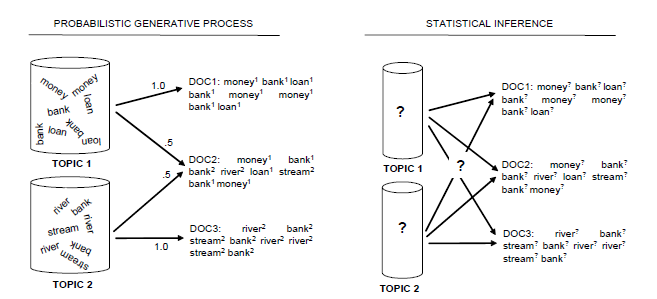
\includegraphics[scale=0.75]{static/figures/model.png}}
    \caption{Απεικόνιση γενετικής διαδικασίας και του προβλήματος στατιστικής συμπερασματολογίας 
    που λύνεται με μοντέλα θεμάτων.}
    \label{fig:ldamodel01}
\end{figure}

Στο σύστημά μας εφαρμόζουμε το \textbf{{\en {LDA (Latent Dirichlet Allocation)}}} ως το μοντέλο για την ανακάλυψη κρυμμένων θεμάτων 
και αναπαριστούμε την κατανομή θεμάτων ως ένα διάνυσμα κάθε εγγραφή του οποίου δηλώνει το βάρος της αντίστοιχης λέξης. 
Για την εφαρμογή του {\en {LDA}} μοντέλου γίνεται χρήση της βιβλιοθήκης {\en {gensim}} \cite{Lda01} της {\en {Python}}. \\

Ο αλγόριθμος ανάλυσης κειμένων {\en {LDA}} αποτελεί ένα πιθανοτικό μοντέλο που επιτρέπει την
ερμηνεία κάποιων δεδομένων μέσα από κάποια σύνολα παρατηρήσεων. 
Για παράδειγμα, αν οι παρατηρήσεις είναι λέξεις που έχουν συλλεχθεί από κάποια κείμενα, 
ο αλγόριθμος θεωρεί ότι τα κείμενα αντιπροσωπεύονται από τυχαίες προσμείξεις
κρυφών θεμάτων, όπου κάθε θέμα χαρακτηρίζεται από μία κατανομή ως προς τις λέξεις.
% κάθε κείμενο είναι μία ανάμειξη από έναν μικρό αριθμών θεμάτων. 
Ο {\en {LDA}} είναι ένα παράδειγμα μοντέλου θεμάτων και παρουσιάστηκε για πρώτη φορά ως γενετικό
μοντέλο ανακάλυψης θεμάτων από τους {\en {David Blei, Andrew Ng}} και {\en {Michael Jordan}} το 2002.
Κύριο πλεονέκτημα του {\en {LDA}}, καθώς και των παραλλαγών του, είναι ο μεγάλος βαθμός
προσαρμογής τους. Έτσι, μπορούν να εφαρμοστούν και σε διάφορα άλλα προβλήματα που
αντικείμενα απασχόλησης δεν είναι κείμενα λέξεων. Για παράδειγμα, ο αλγόριθμος έχει
χρησιμοποιηθεί στο πεδίο της μηχανική όρασης για ανάλυση εικόνας, στο πεδίο της
βιοπληροφορικής για ανάλυση και ανάκτηση γενετικού κώδικα σε δεδομένα ερευνών κ.α. 
Στόχος μας είναι να βρούμε σύντομες περιγραφές των μελών της συλλογής 
που επιτρέπουν μια αποτελεσματική επεξεργασία μεγάλων συλλογών, 
διατηρώντας τις απαραίτητες στατιστικές σχέσεις που είναι χρήσιμες
για βασικές διεργασίες όπως η περίληψη κειμένου.

\begin{figure}[!ht] \centering
\centerline{
    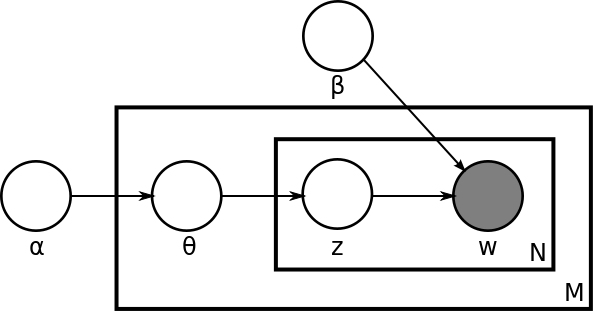
\includegraphics[scale=0.45]{static/figures/ldamodel2.png}}
    \caption{Γραφικό μοντέλο απεικόνισης του {\en {LDA}}. Τα πλαίσια απεικονίζουν τις επαναλήψεις. 
    Το εξωτερικό πλαίσιο απεικονίζει τα κείμενα, ενώ το εσωτερικό την επαναληπτική επιλογή των θεμάτων 
    και των λέξεων μέσα σε ένα κείμενο.}
    \label{fig:ldamodel02}
\end{figure}

Το {\en {LDA}} μοντέλο απεικονίζεται ως πιθανοτικό γραφικό μοντέλο στην εικόνα \ref{fig:ldamodel02}. 
Όπως γίνεται αντιληπτό από την εικόνα, υπάρχουν τρία επίπεδα στο {\en {LDA}}. 
Οι παράμετροι α και β είναι επιπέδου σώματος παράμετροι, που έχουν συλλεχθεί 
από την διαδικασία δημιουργίας του σώματος. 
Οι μεταβλητές θ είναι επιπέδου κειμένου μεταβλητές, που έχουν ληφθεί από ένα κείμενο. 
Τέλος, οι μεταβλητές {\en {z}} και {\en {w}} είναι επιπέδου λέξεων μεταβλητές και έχουν συλλεχθεί για κάθε λέξη κάθε κειμένου. 
Οι μεταβλητές {\en {M, N}} δηλώνουν αντίστοιχα τον αριθμό των κειμένων και τον αριθμό των λέξεων μέσα σε ένα κείμενο.

Είναι απαραίτητο να ξεχωρίσουμε το {\en {LDA}} από το απλό {\en {Dirichlet}} πολυωνυμικό μοντέλο ομαδοποίησης. 
Ένα κλασσικό μοντέλο ομαδοποίησης θα ήταν ένα δύο-επιπέδων μοντέλο, 
όπου η {\en {Dirichlet}} θα υπολογιζόταν μία φόρα για ένα σώμα, μια πολυωνυμική μεταβλητή
ομαδοποίησης θα επιλεγόταν για κάθε κείμενο του σώματος και ένα σύνολο λέξεων
θα επιλεγόταν για ένα κείμενο της μεταβλητής ομάδας. Όπως και με πολλά αλλά μοντέλα
ομαδοποίησης, ένα τέτοιο μοντέλο περιορίζει ένα κείμενο στο να συσχετίζεται μόνο με ένα θέμα. 
Αντιθέτως, το {\en {LDA}} είναι μοντέλο τριών επιπέδων και ο θεματικός κόμβος επιλέγεται επαναλαμβανόμενα από κάθε κείμενο. 
Με αυτό το μοντέλο τα κείμενα μπορούν να συσχετιστούν με πολλά θέματα. \\

\nocite{RecommendLda, Lda03, Scenepaper, Exp01, Hybrid, Adapt, Mining}

Στο σημείο αυτό, έχοντας αναλύσει το θεωρητικό υπόβαθρο γύρω από τα πιθανοτικά θεματικά μοντέλα και συγκεκριμένα το μοντέλο {\en {LDA}}, 
προχωράμε στην εφαρμογή του {\en {LDA}} σε κάθε {\en {cluster}} (κατηγορία) άρθρων, σε κάθε {\en {group}} εντός των {\en {clusters}}, 
καθώς και σε κάθε μεμονωμένο άρθρο.
Έτσι, καταλήγουμε με το διάνυσμα της κατανομής θεμάτων τόσο για τα άρθρα, όσο και για τα {\en {clusters}} και τα {\en {groups}} που έχουν δημιουργηθεί. 
Κάθε καταχώρηση ενός τέτοιου διανύσματος θεμάτων αποτελείται από μία αντιπροσωπευτική λέξη και το αντίστοιχο βάρος. 
Κατά την εφαρμογή του αλγορίθμου μπορούμε να επιλέξουμε τον αριθμό αντιπροσωπευτικών λέξεων απ'τις οποίες θα αποτελείται ένα τέτοιο διάνυσμα. 
% Στο κώδικά μας επιλέξαμε να κρατάμε τις σαράντα πιο κατάλληλες λέξεις για κάθε {\en {cluster, group}} και άρθρο, μαζί με τα αντίστοιχα βάρη τους. 

% **********************************************************
\subsection{Υποσύστημα Δημιουργίας Προφίλ Χρήστη}
% **********************************************************

Ένα από τα ιδιαίτερα χαρακτηριστικά ενός συστήματος δημιουργίας εξατομικευμένων
συστάσεων είναι το Προφίλ Χρήστη (στο πλαίσιο των συστημάτων συστάσεων). Το
Προφίλ Χρήστη είναι μια αναπαράσταση των πληροφοριών που υπάρχουν για ένα
χρήστη, οι οποίες είναι απαραίτητες για ένα προσαρμοζόμενο σύστημα ώστε αυτό να
προσφέρει εξατομίκευση, δηλαδή να συμπεριφέρεται διαφορετικά για διαφορετικούς
χρήστες. \\

Παραδοσιακά, το προφίλ ενός χρήστη μπορεί να καθοριστεί παρακολουθώντας τα άρθρα 
τα οποία έχουν διαβαστεί από το χρήστη μέχρι στιγμής (ιστορικό περιήγησης), με βάση το περιεχόμενο των άρθρων. 
Ο τρόπος αναπαράστασης του προφίλ εξαρτάται από τη μέθοδο που χρησιμοποιεί το σύστημα πρόσβασης.
Ουσιαστικά, το προφίλ αποτελεί ένα σύνολο των πιθανών ενδιαφερόντων του χρήστη.
Παρ\textquotesingleόλ\textquotesingleαυτά, η προσέγγιση αυτή δεν αποτυπώνει αποτελεσματικά τις ακριβείς αναγνωστικές προτιμήσεις του χρήστη, 
καθώς το ενδιαφέρον του ενδέχεται να επηρεάζεται και από τις προτιμήσεις άλλων χρηστών. 
Επιπρόσθετα, η ανεπάρκεια της προσέγγισης στηριζόμενης αποκλειστικά στο περιεχόμενο των άρθρων 
οφείλεται και στο γεγονός ότι πολλοί χρήστες τείνουν να επιλέγουν άρθρα επηρεασμένοι 
από φράσεις/ονοματισμένες οντότητες όπως οι εξής: Τι συνέβη, ποιος εμπλέκεται, πότε συνέβη κ.λπ. \\

Στηριζόμενοι στην παραπάνω ανάλυση, το Προφίλ Χρήστη παραμετροποιείται μέσω μιας τριπλέτας {\en {\textit{U = $\langle$T, P, E $\rangle$}}} 
αποτελούμενης από τα εξής χαρακτηριστικά: 
\begin{itemize}
\item Το {\en {\textit{T}}} αναπαριστά την κατανομή των θεμάτων των ειδησεογραφικών άρθρων τα οποία ο χρήστης έχει διαβάσει στο παρελθόν, 
με μορφή διανύσματος θεμάτων {\en {\textit{\{$\langle$t1, w1$\rangle$, $\langle$t2, w2$\rangle$, ...\}}}}, όπου κάθε καταχώρηση του διανύσματος 
αποτελείται από μια αντιπροσωπευτική λέξη και το αντίστοιχο βάρος. 
\item Το {\en {\textit{P}}} δηλώνει μια λίστα χρηστών {\en {\textit{\{$\langle$u1, u2, ...$\rangle$\}}}} οι οποίοι έχουν παρόμοια πρότυπα πρόσβασης.
\item Το {\en {\textit{E}}} είναι μια λίστα από ονοματισμένες οντότητες {\en {\textit{\{$\langle$e1, e2, ...$\rangle$\}}}} εξαγόμενες από 
το ιστορικό αναγνωσμένων άρθρων του χρήστη, συσχετισμένες με τον αντίστοιχο τύπο οντότητας. 
\end{itemize}

Τα παραπάνω χαρακτηριστικά προφανώς αλληλεπιδρούν μεταξύ τους. Η κατανομή θεμάτων των ειδησεογραφικών άρθρων που εξάγονται απ'το ιστορικό 
ανάγνωσης του χρήστη είναι πολύ πιθανό να συνδέεται με τη λίστα ονοματισμένων οντοτήτων του προφίλ, ενώ αυτά τα δύο χαρακτηριστικά 
ενδέχεται να συνεισφέρουν και στα παρόμοια πρότυπα πρόσβασης δύο χρηστών. \\

% *************
Κάθε ενέργεια που πραγματοποιεί ο χρήστης στο δικτυακό τόπο καταγράφεται στο ιστορικό του,
η ανάλυση του οποίου οδηγεί στην εξαγωγή συμπερασμάτων προκειμένου το σύστημα να μπορεί
να διαμορφώνει αυτόματα το Προφίλ Χρήστη, ώστε να εφαρμοστούν με μεγαλύτερη ακρίβεια 
οι τεχνικές εξατομίκευσης και κατ\textquotesingleεπέκταση οι προτεινόμενες συστάσεις. \\

Παρακάτω αναλύουμε λεπτομερώς τις τεχνικές που υιοθετήθηκαν για την κατασκευή διαφορετικών πτυχών του προφίλ του χρήστη: 
\begin{itemize}
 \item \textbf{Σύνοψη Θεματικού Περιεχομένου Αναγνωσμένων Άρθρων}: \\ 
 Στο σύστημα συστάσεων που υλοποιήσαμε συνοψίζουμε τα ειδησεογραφικά άρθρα του ιστορικού του χρήστη ως κατανομή θεμάτων, 
χρησιμοποιώντας την ίδια στρατηγική που εφαρμόσαμε και για τον εντοπισμό ειδησεογραφικών θεμάτων μέσω πιθανοτικών θεματικών μοντέλων  
στα {\en {clusters}} άρθρων της βάσης δεδομένων του συστήματος. 
Ουσιαστικά, χρησιμοποιούμε την ίδια αναπαράσταση του ιστορικού αναγνωσμένων άρθρων του χρήστη 
με αυτή των {\en {clusters}} άρθρων.

% ---------------------------------------------------
 \item \textbf{Ανάλυση Προτύπων Πρόσβασης}: \\ 
 Στην πραγματικότητα πολλοί αναγνώστες διαδικτυακών άρθρων επιδεικνύουν παρόμοιες αναγνωστικές προτιμήσεις. 
Το προφίλ ενός χρήστη μπορεί να εμπλουτιστεί αναλύοντας τις αναγνωστικές προτιμήσεις άλλων χρηστών παρόμοιων 
με το δεδομένο χρήστη και ενσωματώνοντάς τες σε αυτό. Συγκεκριμένα, αναλύουμε το ιστορικό αναγνωσμένων άρθρων 
όλων των χρηστών του συστήματος. Υποθέτοντας ότι οι συλλογές άρθρων που αναγνώστηκαν από τους χρήστες  {\en {\textit{A}}} 
και  {\en {\textit{B}}} είναι οι  {\en {\textit{$N_A$}}} και  {\en {\textit{$N_B$}}}, η ανά ζεύγος ομοιότητα των προτύπων πρόσβασης 
ορίζεται ως η {\en {Jaccard}} ομοιότητα μεταξύ των συνόλων {\en {\textit{$N_A$}}} και  {\en {\textit{$N_B$}}}. 
Η ομοιότητα {\en {Jaccard}} για δύο σύνολα είναι το μέγεθος της τομής προς το μέγεθος της ένωσής τους \cite{Jac02}. 

Υπολογίζοντας τις ανά ζεύγος ομοιότητες μεταξύ των χρηστών του συστήματος, δημιουργούμε ένα διάνυσμα ομοιοτήτων, 
κάθε εγγραφή του οποίου αποτελεί την {\en {Jaccard}} ομοιότητα μεταξύ των προτύπων πρόσβασης δύο χρηστών. 
Δεδομένου ενός χρήστη {\en {\textit{u}}}, κάθε άλλος χρήστης μπορεί να θεωρηθεί όμοιός του αν το ανά ζεύγος σκορ ομοιότητάς τους 
ξεπερνά ένα προκαθορισμένο κατώφλι {\en {\textit{$t_u^2$}}}. 

Η ανάλυση προτύπων πρόσβασης οδηγεί στην εξαγωγή μιας λίστας με τα ονόματα παρόμοιων χρηστών για κάθε χρήστη. 
Η πληροφορία αυτή αποθηκεύεται στη βάση δεδομένων και ενημερώνεται καθ'όλη τη διάρκεια περιήγησης του κάθε χρήστη στο σύστημα, 
καθότι κάθε νέο άρθρο που επιλέγεται προς ανάγνωση, μετατρέπει άμεσα τον εκάστοτε χρήστη σε λιγότερο ή περισσότερο όμοιο με κάποιον άλλο χρήστη. 

% ---------------------------------------------------
 \item \textbf{Εξαγωγή Ονοματισμένων Οντοτήτων}: \\ 
 Τυπικά, στα ειδησεογραφικά άρθρα οι ονοματισμένες οντότητες περιλαμβάνουν λέξεις/φράσεις όπως “πότε, πού, τι συνέβη, ποιος εμπλέκεται” κ.λπ. 
Οι αναγνώστες ενδέχεται να έχουν προτίμηση σε κάποιες συγκεκριμένες ονοματισμένες οντότητες ενός άρθρου. Συνεπώς, οι οντότητες αυτές 
είναι σημαντικές για ένα σύστημα που θέλει να προσφέρει εξατομικευμένες συστάσεις σε χρήστες. 

Για την εξαγωγή των ονοματισμένων οντοτήτων χρησιμοποιήσαμε το ανοιχτού κώδικα εργαλείο επεξεργασίας φυσικής γλώσσας 
{\en {GATE (General Architecture for Text Engineering)}}, το οποίο αναγνωρίζει αυτόματα ονοματισμένες οντότητες σε κείμενα, δεδομένων 
κάποιων κανόνων. Για τη συγκεκριμένη διαδικασία χρησιμοποιήσαμε τους προεπιλεγμένους κανόνες του εργαλείου. 

Κατά την προεπεξεργασία των κειμένων, έχοντας εξάγει το κείμενο κάθε άρθρου της βάσης δεδομένων σε αρχείο κειμένου, 
φορτώνουμε όλα τα αρχεία στο {\en {GATE}} και προχωρούμε στη δημιουργία ενός {\en {corpus}} κειμένων. 
Τρέχουμε το {\en {dictionary-based Named Entity Recognition}} εργαλείο {\en {ANNIE Gazetteer}} με είσοδο το {\en{corpus}} κειμένων 
και επιλέγουμε την εξαγωγή του κειμένου κάθε άρθρου σε μορφή {\en {.xml}} \cite{Gt02}.
Με κατάλληλη επεξεργασία των {\en {.xml}} αρχείων κρατάμε την πληροφορία των ετικετών που μας ενδιαφέρουν (ονόματα, τοποθεσίες και οργανισμοί), 
κάνοντας χρήση της βιβλιοθήκης {\en {Beautiful Soup}} \cite{Bs01} της {\en {Python}}. 

Η πληροφορία που εξάγεται για κάθε άρθρο, δηλαδή το όνομα της οντότητας μαζί με τον αντίστοιχο τύπο της {\en {(Organization, Person, Location)}}, 
αποθηκεύεται στη βάση δεδομένων του συστήματος. 
Μετά την αναγνώριση των οντοτήτων, κάθε άρθρο συσχετίζεται με μία λίστα από ονοματισμένες οντότητες μαζί με τον αντίστοιχο τύπο. 
Έτσι, είναι εύκολο να εξάγουμε τις ονοματισμένες οντότητες που αφορούν τον εκάστοτε χρήστη, 
ανατρέχοντας κάθε φορά στο ιστορικό αναγνωσμένων άρθρων, εξάγοντας τις αποθηκευμένες οντότητες για τα άρθρα αυτά 
και ανανεώνοντας την εν λόγω λίστα με τις οντότητες των άρθρων αυτών. 

\end{itemize}

\begin{comment}
\end{comment}

% **********************************************************
\subsection{Υποσύστημα Προσωποποιημένων Συστάσεων}
% **********************************************************

Στο τελευταίο στάδιο του προτεινόμενου συστήματος παρέχονται εξατομικευμένες συστάσεις σε μεμονωμένους χρήστες. 
Η εξατομικευμένη σύσταση ειδησεογραφικών άρθρων στηρίζεται στη διερεύνηση της σχέσης μεταξύ 
πρόσφατα δημοσιευμένων άρθρων και του προφίλ του χρήστη. 
Στην παρούσα διπλωματική εργασία προτάθηκε η χρήση μιας υβριδικής μεθόδου συστάσεων. 
Ωστόσο, η διαφοροποίηση από προηγούμενες προσεγγίσεις έγκειται στην πρόταση για διεπίπεδη ιεραρχία συστάσεων, 
όπου το πρώτο επίπεδο δείχνει μια σύντομη σύνοψη για κάθε κατηγορία θεμάτων που μπορεί να προτιμά ο χρήστης και
το δεύτερο επίπεδο δίνει μια συγκεκριμένη λίστα με άρθρα ειδήσεων παρόμοια με το αναγνωστικό ενδιαφέρον του χρήστη. 

% ____________________________________________
\subsubsection{Αντιστοίχιση Αναγνωστικών Προτιμήσεων για την Αναπαράσταση 1ου Επιπέδου} 
% ____________________________________________
Αφού δημιουργήσουμε την ιεραρχία των ειδησεογραφικών άρθρων (συσταδοποίηση σε {\en {clusters}} και {\en {groups}} εντός αυτών), 
καθώς και το προφίλ του χρήστη, 
το πρώτο επίπεδο αναπαράστασης μπορεί να επιτευχθεί με τη διαδοχική αντιστοίχιση του προφίλ του χρήστη στην ιεραρχία ειδήσεων 
και την επιλογή των κατάλληλων {\en {clusters}}. 
Σημειώνουμε ότι κάθε {\en {cluster}} αντιστοιχίζεται σε μία κατηγορία θεμάτων. \\
% Για λόγους απλότητας λαμβάνουμε υπόψιν μόνο την ομοιότητα μεταξύ των κατανομών θεμάτων κάθε ενδιάμεσης ομάδας 
% και του αναγνωστικού ιστορικού του χρήστη. \\

Τυπικά, η κατανομή θεμάτων αναπαρίσταται ως ένα διάνυσμα θεμάτων {\en {\textit{T = \{$\langle$t1, w1$\rangle$, $\langle$t2, w2$\rangle$, ...\}}}}. 
Για να εξασφαλίσουμε ότι όλα τα διανύσματα θεμάτων έχουν την ίδια διάσταση, δημιουργούμε 
ένα λεξιλόγιο θεμάτων {\en {\textit{V}}} βασισμένο στα ήδη υπάρχοντα θέματα, όπου {\en {\textit{$\vert V\vert$}}} 
είναι ο συνολικός αριθμός από αντιπροσωπευτικές λέξεις. 
Κάθε διάσταση αντιστοιχεί σε μία ξεχωριστή λέξη. Αν η λέξη υπάρχει μέσα στο κείμενο, η τιμή του διανύσματος δεν είναι μηδενική. 
Συγκρίνουμε το βαθμό ομοιότητας της κατανομής θεμάτων κάθε ομάδας, {\en {\textit{$T_C$}}}, με αυτή του προφίλ του χρήστη, {\en {\textit{$T_U$}}}, 
μέσω της ομοιότητας συνημιτόνου {\en {(cosine similarity)}} \cite{Cs01}. \\

{\textbf {\textit{Ομοιότητα  Συνημιτόνου:}}} 
Οι προς σύγκριση κατανομές θεμάτων αναπαρίστανται ως διανύσματα σε ένα πολυδιάστατο χώρο. 
Η μετρική ομοιότητας συνημιτόνου υπολογίζει την ομοιότητα από το συνημίτονο της γωνίας που σχηματίζουν 
τα δύο διανύσματα. Η ελάχιστη τιμή της μετρικής είναι {\textit{-1}}, υποδηλώνοντας την απόκλιση 
των διανυσμάτων και η μέγιστη {\textit{1}}, υποδηλώνοντας την απόλυτη ταύτιση. 
Όταν τα διανύσματα είναι κάθετα μεταξύ τους και σχηματίζουν γωνία 90$^{\circ}$, το συνημίτονο είναι {\textit{0}}, 
υποδηλώνοντας ότι τα διανύσματα είναι ανεξάρτητα. \\

Η εξίσωση που εφαρμόζουμε για τον υπολογισμό της μετρικής αυτής είναι η ακόλουθη:

\begin{equation}
{\en {Sim(\pmb T_C, \pmb T_U) = \frac{\pmb T_C \cdot \pmb T_U}{||\pmb T_C|| ||\pmb T_U||} }}
\end{equation}

όπου \begin{math} {\en {|\pmb T_C| = |\pmb T_U| = |\pmb V|}}\end{math}, 
και \begin{math} {\en {||\pmb T_C||, ||\pmb T_U||}} \end{math} αποτελούν τις {\en {l2}}-νόρμες. \\

Η κατάταξη των {\en {clusters}} βασίζεται στο σκορ ομοιότητας 
που υπολογίζεται από την εξίσωση (2.1). 
Γενικά, οι χρήστες τείνουν να προτιμούν συγκεκριμένες κατηγορίες θεμάτων, 
χωρίς να ενδιαφέρονται για όλα τα θέματα. 
Ως εκ τούτου, επιλέγουμε τα {\en {clusters}} με σκορ ομοιότητας μεγαλύτερο από ένα δυναμικό κατώφλι. 
Αφού επιλέξουμε τα κατάλληλα {\en {clusters}}, εισχωρούμε σε κάθε {\en {cluster}} και επιλέγουμε 
το {\en {group}} νέων που είναι πιο κοντά σε ομοιότητα με τις προτιμήσεις του χρήστη, 
κάνοντας χρήση της ίδιας στρατηγικής μέσω της οποίας επιλέξαμε και τα {\en {clusters}} προηγουμένως. 
Έτσι, δημιουργείται μια λίστα από {\en {group}} άρθρων (ένα {\en {group}} από κάθε {\en {cluster}}), η οποία και επιλέγεται ως η βάση 
για το δεύτερο επίπεδο σύστασης. 
% Από την αλληλεπίδραση των χρηστών με το σύστημα γίνεται άμεσα αντιστοίχιση των χρηστών σε θέματα που τους ενδιαφέρουν.

% ____________________________________________
\subsubsection{Αντιστοίχιση Αναγνωστικών Προτιμήσεων για την Αναπαράσταση 2ου Επιπέδου} 
% ____________________________________________
Έχοντας εξασφαλίσει τα {\en {group}} άρθρων που πιθανότατα ενδιαφέρουν το χρήστη, 
το ακόλουθο βήμα είναι η επιλογή συγκεκριμένων άρθρων προς αναπαράσταση στο χρήστη. 
Αρχικά, διαμορφώνουμε ένα προφίλ για κάθε ειδησεογραφικό άρθρο και εν συνεχεία, 
μοντελοποιούμε τις προσωποποιημένες συστάσεις ως ένα “προϋπολογισμένο πρόβλημα μέγιστης κάλυψης”
{\en {(budgeted maximum coverage problem)}} \cite{Bm01} και το επιλύουμε μέσω ενός άπληστου {\en {(greedy)}} προσεγγιστικού αλγορίθμου. \cite{Sub01} \\

%\paragraph{Δημιουργία Προφίλ Ειδησεογραφικών Άρθρων} 
\textbf{Δημιουργία Προφίλ Ειδησεογραφικών Άρθρων} 

Ένα ειδησεογραφικό άρθρο αποτελείται από στατικά χαρακτηριστικά (π.χ. κατανομή θεμάτων, 
ονοματισμένες οντότητες) και δυναμικά χαρακτηριστικά (π.χ. χρήστες που το διάβασαν, δημοφιλία, 
πόσο “φρέσκο” είναι από τη σκοπιά του πόσο πρόσφατα δημοσιεύθηκε). 
Σχετικά με τα στατικά χαρακτηριστικά, η κατανομή θεμάτων κάθε άρθρου καθώς και οι ονοματισμένες οντότητές του 
έχουν εξαχθεί σε προηγούμενο βήμα της εφαρμογής και βρίσκονται ήδη αποθηκευμένα σε αντίστοιχους πίνακες της βάσης δεδομένων του συστήματος. 
Σχετικά με τη δημοφιλία, υπολογίζουμε το λόγο των χρηστών που το διάβασαν 
προς το συνολικό αριθμό χρηστών του συστήματος. 
Σχετικά με το πόσο πρόσφατα δημοσιεύθηκε, υπολογίζουμε τη διαφορά μεταξύ της ημερομηνίας δημοσίευσης 
και της τρέχουσας ημερομηνίας. \\

Στο σύστημά μας, τα προφίλ των άρθρων είναι ιδιαιτέρως βοηθητικά στο να συγκρίνουμε μεταξύ τους 
δύο άρθρα και να μπορέσουμε να αξιολογήσουμε σε τι βαθμό ικανοποιεί το καθένα εξ αυτών 
τις αναγνωστικές προτιμήσεις του χρήστη. 
Οι δύο παραπάνω συγκρίσεις, αυτή μεταξύ προφίλ άρθρων και αυτή μεταξύ προφίλ άρθρου και προφίλ χρήστη 
υπολογίζονται μέσω της ίδια φόρμουλας. \\

Δεδομένων ενός προφίλ άρθρου {\en {\textit{$F_n$ = $\langle T_n, P_n, E_n \rangle$}}}
και ενός προφίλ χρήστη {\en {\textit{$F_u$ = $\langle T_u, P_u, E_u \rangle$}}}, 
η ομοιότητα μεταξύ των {\en {\textit{$F_n$}}} και {\en {\textit{$F_u$}}} υπολογίζεται ως εξής: 

\begin{figure}[!ht] \centering
    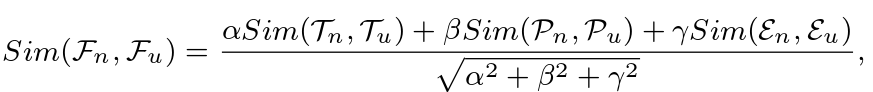
\includegraphics[scale=0.4]{static/figures/sim.png}
    \label{}
\end{figure} 

όπου {\en {\textit{a, b}}} και {\en {\textit{c}}} είναι παράμετροι μέσω των οποίων 
ρυθμίζουμε το πόσο εμπιστευόμαστε τα αντίστοιχα μέρη. 
Στο δικό μας σύστημα συστάσεων επιλέγουμε να αναθέσουμε ίση σημαντικότητα 
σε κάθε έναν από τους παραπάνω παράγοντες, δεδομένου ότι αναπαριστούν διαφορετικές 
αλλά, παράλληλα, συνδεδεμένες πτυχές ενός ειδησεογραφικού άρθρου ή ενός προφίλ χρήστη, 
αναθέτοντας και στους τρεις παράγοντες την ίδια τιμή {\en {\textit{a = b = c = 1}}}. \\

Η {\en {\textit{Sim($T_C, T_U$)}}} υπολογίζεται μέσω της εξίσωσης (2.1), 
ενώ οι {\en {\textit{Sim($P_n, P_u$)}}} και 
{\en {\textit{Sim($E_n, E_u$)}}} 
υπολογίζονται μέσω της ομοιότητας {\en {Jaccard}}. 
Η ομοιότητα {\en {Jaccard}} \cite{Jac02} για δύο σύνολα είναι το μέγεθος της τομής προς το μέγεθος της ένωσής τους. \\

%--------------------------------
\textbf{Εισαγωγή στις {\en {Submodular}} Συναρτήσεις}

Μια κατηγορία συναρτήσεων που χρησιμοποιούνται ευρέως 
και παρουσιάζουν ιδιαίτερο ενδιαφέρον είναι οι {\en {submodular}} συναρτήσεις. 
Οι συναρτήσεις αυτές προσπαθούν να μοντελοποιήσουν το γεγονός ότι 
όσο συνεχίζουμε να δίνουμε αγαθά σε κάποιον χρήστη, 
επέρχεται ένας κορεσμός στην ωφέλειά του. 
Η αύξηση της ωφέλειας από την απόκτηση νέων αγαθών είναι μικρή όταν ο χρήστης έχει ήδη στην κατοχή του κι άλλα αγαθά. 
Έχουμε, λοιπόν, μια μονότονη (φθίνουσα) συμπεριφορά στην αύξηση της ωφέλειας. \\

\textbf{Ορισμός.} Μια συνάρτηση ωφέλειας {\en {f}} για έναν χρήστη {\en {i}} είναι {\en {submodular}} 
αν για οποιαδήποτε δύο υποσύνολα αντικειμένων \textit{{\en {S, T}}}, με \textit{{\en {S}}} $\subseteq$ \textit{{\en {T}}}, 
και για κάθε αντικείμενο \textit{{\en {j}}} $\notin$ \textit{{\en {T}}}, ισχύει ότι 

\begin{figure}[!ht] \centering
    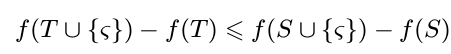
\includegraphics[scale=0.55]{static/figures/modul.png}
    \label{}
\end{figure} 

Ο παραπάνω ορισμός μάς λέει ότι η αύξηση της ωφέλειας που προκαλεί η προσθήκη του αγαθού $\varsigma$ στον χρήστη {\en {i}} 
είναι μεγαλύτερη όταν προσθέτουμε το $\varsigma$ σε ένα σύνολο αγαθών {\en {S}}, από ότι όταν το προσθέτουμε σε ένα 
μεγαλύτερο σύνολο του {\en {S}} (το {\en {T})}. Πάρα πολλά μικροοικονομικά μοντέλα στηρίζονται στην υπόθεση ότι οι 
εμπλεκόμενοι χρήστες έχουν {\en {submodular}} συμπεριφορά. Κλασικό παράδειγμα αποτελούν και τα κοινωνικά δίκτυα, 
όπου η προσθήκη ενός νέου φίλου θα αυξήσει περισσότερο την κοινωνική επιρροή σε μία λιγότερο κοινωνική ομάδα 
από ό,τι σε μία πιο κοινωνική. \\

Μία πιο μαθηματική διατύπωση για το πρόβλημα της μεγιστοποίησης της επιρροής είναι η εξής: 
δεδομένου ενός συνόλου στοιχείων $E$, όπου κάθε στοιχείο είναι συσχετισμένο με μία τιμή επιρροής και ένα κόστος, 
και δεδομένου, επίσης, ενός {\en {budget}} $B$ άρθρων, ο σκοπός είναι να βρεθεί ένα υποσύνολο του $E$ όπου θα 
μεγιστοποιεί την επιρροή (δηλαδή την συνάρτηση {\en {$f(S)$}}) χωρίς το συνολικό κόστος να ξεπερνά το {\en {budget}} $B$. 
Ως {\en {budget}} B μπορεί να θεωρηθεί ο μέγιστος αριθμός από προτεινόμενα άρθρα μέσα σε κάθε {\en {group}} άρθρων. 
Το πρόβλημα της μεγιστοποίησης της επιρροής είναι δυστυχώς {\en {NP-hard}}. 
Ωστόσο, το επιλύουμε μέσω ενός άπληστου {\en {(greedy)}} προσεγγιστικού αλγορίθμου, 
ο οποίος επιλέγει διαδοχικά το στοιχείο το οποίο αυξάνει τη μέγιστη δυνατή επιρροή εντός του ορίου κόστους. 
Δηλαδή προσθέτουμε κάθε φορά στο {\en {S}} το άρθρο που σε αυτό το σημείο μεγιστοποιεί το οριακό κέρδος {\en {(marginal gain)}}.
Ο αλγόριθμος αυτός αποδεικνύεται ότι αποτελεί ($1 - \frac{1}{e})$-προσέγγιση του βέλτιστου, δηλαδή προσέγγιση του βέλτιστου κατά 63\%. \\

\begin{algorithm}
\begin{algorithmic}
 \STATE {\en {Start with an empty set $S$}}
 {\en{
 \FOR {\en{{B iterations}}}
  \STATE {\en {Add article $\varsigma$ to $S$ so that it maximizes $I$($\varsigma$) = $f(S$ $\cup$ \{$\varsigma$\}) - $f(S)$}}
  \ENDFOR }}
\end{algorithmic}
\caption{Άπληστος προσεγγιστικός αλγόριθμος}
\end{algorithm}


%--------------------------------
\textbf{{\en {Submodularity}} Μοντέλο Συστάσεων}

Με βάση τη συγκεκριμένη στρατηγική, ορίζουμε μία συνάρτηση ποιότητας {\en {$f$}} 
για να αξιολογήσουμε το επιλεγμένο σετ άρθρων {\en {$S$}} σε σχέση με ολόκληρο το 
{\en {group}} νέων {\en {$N$}} ως εξής: 

\begin{figure}[!ht] \centering
    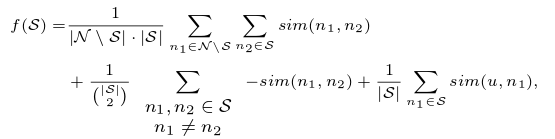
\includegraphics[scale=0.6]{static/figures/quality.png}
    \label{}
\end{figure} 

όπου {\en {$n_1$}} και {\en {$n_2$}} υποδηλώνουν άρθρα, το {\en {$u$}} αναπαριστά 
τον δεδομένο χρήστη και η {\en {$sim(.,.)$}} αναπαριστά την ομοιότητα μεταξύ των δύο προφίλ, 
είτε αναφερόμαστε σε προφίλ χρήστη είτε σε προφίλ άρθρου. \\

Η παραπάνω εξίσωση αποτελείται από τρία μέρη: \\
Το πρώτο στοχεύει στην εκτίμηση της ποιότητας του πόσο αντιπροσωπευτικό είναι το επιλεγμένο σετ νέων $S$, 
το δεύτερο παρέχει μία εικόνα για το πόσο ποικίλα είναι τα θέματα που κρύβονται στα επιλεγμένα άρθρα και τέλος, 
το τρίτο μέρος μάς δίνει στοιχεία για το πόσο ικανοποιούνται οι προτιμήσεις του χρήστη από το επιλεγμένο σετ $S$. 
Η συνάρτηση {\en {$f(S)$}} εξισορροπεί τη συνεισφορά κάθε ενός μέρους. 
Και τα τρία αυτά μέρη αποτελούν {\en {submodular}} συναρτήσεις, άρα είναι μη αρνητικές και μονότονες, 
επομένως και η συνάρτηση {\en {$f(S)$}} θα είναι {\en {submodular}}. \\
Υποθέτοντας ότι το άρθρο $\varsigma$ είναι το υποψήφιο άρθρο, η αύξηση της ωφέλειας αναπαρίσταται ως εξής: 

\begin{figure}[!ht] \centering
    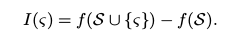
\includegraphics[scale=0.7]{static/figures/increase.png}
    \label{}
\end{figure} 

Στόχος είναι να βρεθεί μία λίστα από άρθρα η οποία μεγιστοποιεί το οριακό κέρδος εντός του δοσμένου {\en {budget}}.
Έτσι, μοντελοποιούμε τις προσωποποιημένες συστάσεις άρθρων ως ένα “προϋπολογισμένο πρόβλημα μέγιστης κάλυψης”. \\

Αρχικά, φροντίζουμε να αφαιρέσουμε από κάθε επιλεγμένο {\en {group}} άρθρων τα άρθρα τα οποία βρίσκονται ήδη 
στο ιστορικό ανάγνωσης του χρήστη, καθώς άρθρα που έχουν ήδη αναγνωσθεί δεν πρέπει να βρεθούν στην τελική προτεινόμενη λίστα. 
Έτσι, καταλήγουμε με μία λίστα από λίστες, κάθε μία εκ των οποίων περιλαμβάνει 
τα εναπομείναντα υποψήφια προς πρόταση άρθρα από κάθε {\en {group}}. \\
Στη συνέχεια, υπολογίζουμε το {\en {budget}} για κάθε λίστα, 
δηλαδή το μέγιστο αριθμό προτεινόμενων άρθρων από κάθε κατηγορία που επιλέχθηκε ως ταιριαστή με τις προτιμήσεις του χρήστη. 
Το {\en {budget}} υπολογίζεται με βάση την ομοιότητα κάθε χρήστη με το εν λόγω {\en {cluster}}/κατηγορία. 
Όσο μεγαλύτερη είναι η τιμή που προκύπτει από τη σύγκριση μεταξύ των κατανομών θεμάτων χρήστη και του εκάστοτε {\en {cluster}}, 
τόσο μεγαλύτερος είναι ο αριθμός άρθρων που επιλέγονται να προταθούν από την εν λόγω κατηγορία άρθρων. \\
Στο σημείο αυτό προβήκαμε σε μία παραδοχή:  
Η εφαρμογή του άπληστου αλγορίθμου {\en {(Algorithm 1)}} σε κάθε {\en {group}} άρθρων (προκειμένου να επιλύσουμε 
το πρόβλημα μέγιστης κάλυψης, επιλέγοντας διαδοχικά το άρθρο που προσφέρει τη μέγιστη αύξηση ωφέλειας από το επιλεγμένο σετ $S$, 
μέσα στο πλαίσιο που ορίζεται από το {\en {budget}}), αποδείχθηκε υπερβολικά χρονοβόρα για ένα τυπικό υπολογιστικό σύστημα 
και ξέφευγε από την ουσία ενός συστήματος συστάσεων. 
Ο χρήστης θα έπρεπε να περιμένει υπερβολικά πολλή ώρα προκειμένου να δεχθεί ως σύσταση τη βέλτιση επιλογή άρθρων, 
όπως θα μας την υποδείκνυε η συνάρτηση αξιολόγησης.
Έτσι, καταφύγαμε στη λύση του να υπολογίσουμε για κάθε {\en {group}} όλους τους δυνατούς συνδυασμούς άρθρων, μεγέθους ίσου με το αντίστοιχο {\en {budget}}, 
και να επιλέξουμε τυχαία έναν από αυτούς μέσω της συνάρτησης {\en {rand}}.
Αν, για παράδειγμα, το {\en {budget}} για ένα {\en {group}} είναι ίσο με την τιμή τρία, τότε υπολογίζουμε όλες τις πιθανές τριάδες άρθρων. \\
Για να ενσωματώσουμε τα προτεινόμενα άρθρα από κάθε {\en {group}} στην τελική προτεινόμενη λίστα, 
επιλέγουμε, λοιπόν, μία τυχαία ν-άδα από κάθε {\en {group}} και όχι απαραίτητα αυτή με την υψηλότερη κατάταξη.
\begin{comment}
Εφαρμόζουμε τον άπληστο αλγόριθμο {\en {(Algorithm 1)}} σε κάθε μία από τις ν-άδες άρθρων 
προκειμένου να επιλύσουμε το πρόβλημα μέγιστης κάλυψης, επιλέγοντας την ν-άδα που προσφέρει τη μέγιστη αύξηση ωφέλειας 
από το επιλεγμένο σετ $S$. \\
Για να ενσωματώσουμε τα προτεινόμενα άρθρα από κάθε {\en {group}} στην τελική προτεινόμενη λίστα, 
επιλέγουμε την ν-άδα με την υψηλότερη κατάταξη από κάθε {\en {group}}.
\end{comment}

\begin{comment}
Εφαρμόζουμε τον άπληστο αλγόριθμο {\en {(Algorithm 1)}} σε κάθε {\en {group}} άρθρων προκειμένου να επιλύσουμε 
το πρόβλημα μέγιστης κάλυψης, επιλέγοντας διαδοχικά το άρθρο που προσφέρει τη μέγιστη αύξηση ωφέλειας από το επιλεγμένο σετ $S$, 
μέσα στο πλαίσιο που ορίζεται από το {\en {budget}}. 
Για να ενσωματώσουμε τα προτεινόμενα άρθρα από κάθε {\en {group}} στην τελική προτεινόμενη λίστα, 
επιλέγουμε τα άρθρα με την υψηλότερη κατάταξη από κάθε {\en {group}}, όπου ο αριθμός των επιλεγμένων άρθρων 
από κάθε {\en {group}} είναι ανάλογος του ενδιαφέροντος του χρήστη για την εν λόγω κατηγορία. \\
\end{comment}

Η {\en {submodularity-based}} στρατηγική επιλογής άρθρων οδηγεί σε μία αρκετά ποικίλη λίστα άρθρων από κάθε κατηγορία. \\
 
%--------------------------------
\textbf{Προσαρμογή Κατάταξης Ειδησεογραφικών Άρθρων} 

Υιοθετώντας τον άπληστο αλγόριθμο που αναλύσαμε νωρίτερα, 
μπορούμε να εξάγουμε μία λίστα από ειδησεογραφικά άρθρα για κάθε θεματική κατηγορία. 
Λαμβάνοντας υπ'όψιν τα αποκλειστικά χαρακτηριστικά των άρθρων, όπως η δημοφιλία και το 
πόσο πρόσφατα δημοσιευμένα είναι, η κατάταξη των επιλεγμένων άρθρων χρειάζεται να προσαρμοστεί 
ώστε να κάνουμε το προτεινόμενο αποτέλεσμα πιο λογικό. \\

Στο σύστημά μας η δημοφιλία ενός άρθρου και το πόσο πρόσφατα δημοσιεύθηκε αποτελούν μέρος του Προφίλ Άρθρου, 
τη δημιουργία του οποίου αναλύσαμε ενδελεχώς σε προηγούμενη παράγραφο. 
Κάνοντας προσαρμογές στη λίστα επιλεγμένων άρθρων, συνδυάζουμε τις κανονικοποιημένες τιμές 
αυτών των δύο τύπων ιδιοτήτων. Τυπικά, δεδομένου ενός άρθρου {\en {$n$}}, 
η δημοφιλία {\en {$n_P$}} και το πόσες μέρες είναι δημοσιευμένο {\en {$n_I$}} 
μπορούν να συνδυαστούν ως εξής: 

\begin{figure}[!ht] \centering
    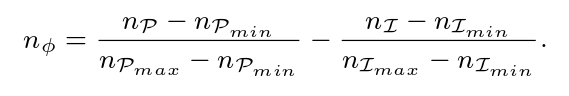
\includegraphics[scale=0.55]{static/figures/comb.png}
    \label{}
\end{figure} 

Παρατηρούμε ότι όσο πιο πρόσφατα δημοσιεύθηκε ένα άρθρο 
(και άρα, όσο πιο μικρή η τιμή του εν λόγω χαρακτηριστικού), 
τόσο υψηλότερη θέση παίρνει το άρθρο στην τελική κατάταξη. 
Δεδομένης μια λίστας άρθρων προς σύσταση, επιλέγουμε διαδοχικά 
δύο γειτονικά άρθρα {\en {$n_i$}} και {\en {$n_j$}} από την κορυφή της λίστας προς τα κάτω 
και τα συγκρίνουμε ως προς το δυναμικό τους σκορ, {\en {$n_f$}}. 
Εάν η εν λόγω διαφορά είναι μεγαλύτερη από μηδέν, ανταλλάσουμε τη θέση των δύο αυτών άρθρων. 
Αλλιώς, τα προσπερνούμε και συνεχίζουμε με τη σύγκριση του επόμενου ζεύγους άρθρων. \\

Μέσω αυτής της μικρής προσαρμογής η παραγόμενη κατάταξη δίνει έμφαση στα πιο δημοφιλή και 
“φρέσκα” ειδησεογραφικά άρθρα, καθώς, επίσης, επικεντρώνεται σε άρθρα που ικανοποιούν σε 
μεγαλύτερο βαθμό τις αναγνωστικές προτιμήσεις του χρήστη. 













